\subsubsection{Modelado de Jeff Jones} % (fold)
\label{ssub:jones}
    El algoritmo propuesto en 'From Pattern Formation to Material Computation: Multi-agent Modelling of Physarum Polycephalum' 
        \cite{Jones2015} aprovecha el comportamiento natural de \textit{Physarum polycephalum} para resolver problemas 
        computacionales mediante un marco de sistema multiagente (MAS). El n\'ucleo del algoritmo involucra un gran n\'umero de 
        agentes simples que imitan el comportamiento del plasmodio de \textit{Physarum}. Cada agente opera basado en reglas 
        locales, movi\'endose e interactuando dentro de un entorno virtual que simula el espacio f\'isico donde reside el moho del limo.
    \vskip 0.5cm
    Los agentes se mueven hacia las fuentes de nutrientes siguiendo gradientes qu\'imicos, representando las se\~nales atrayentes 
        utilizadas por \textit{Physarum}. Dejan rastros similares a feromonas que refuerzan los caminos exitosos, de manera similar 
        a c\'omo \textit{Physarum} fortalece sus tubos protoplasm\'aticos. Este mecanismo de retroalimentaci\'on de feromonas permite 
        que los agentes se adapten din\'amicamente a los cambios en el entorno, optimicen caminos y encuentren soluciones a 
        problemas como el camino m\'as corto o la resoluci\'on de laberintos. El comportamiento colectivo de estos agentes 
        simples conduce a la emergencia de redes complejas y eficientes que pueden ser utilizadas para tareas de computaci\'on no convencional.
    \vskip 0.5cm
    La fortaleza del algoritmo radica en su capacidad de autoorganizaci\'on y adaptaci\'on sin control central. 
        Demuestra capacidades robustas de resoluci\'on de problemas incluso en entornos din\'amicos e inciertos. Al aprovechar 
        los principios de autoorganizaci\'on e interacci\'on local, el algoritmo ofrece un enfoque novedoso para la computaci\'on 
        distribuida y la optimizaci\'on, inspirado en el comportamiento natural de \textit{Physarum polycephalum}.

    % Imagen del pseudoc\'odigo del algoritmo
    \begin{figure}[h]
        \centering
        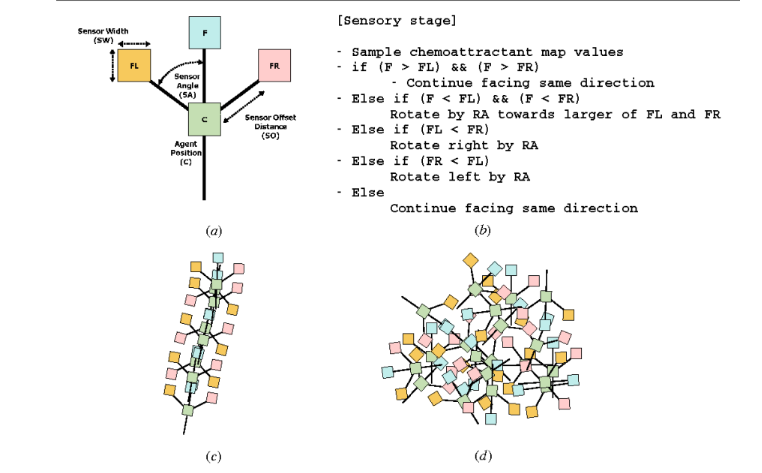
\includegraphics[width=0.7\textwidth]{./images/estado_del_arte/physarum/pseudoJones.png}
        \caption{Representaci\'on del agente de acuerdo con el modelo de Jeff Jones. \cite{Jones2015}}
        \label{fig:pseudocodigo}
    \end{figure}
